% Projekt z předmětů IFJ a IAL
% Author(s): Filip Kocica < xkocic01 AT fit.vutbr.cz>
%
% 29/11/2017

\documentclass[11pt, titlepage, a4paper]{article}
\usepackage[left=1.5cm,text={17cm, 24cm},top=3cm,left=2cm]{geometry}
\usepackage[czech]{babel}
\usepackage[utf8]{inputenc}
\usepackage[T1]{fontenc}
\usepackage{times}
\usepackage[ruled,czech,linesnumbered,longend,noline]{algorithm2e}
\usepackage{algorithmic}
\usepackage{graphicx}
\usepackage{picture}
\usepackage{url}
\usepackage{listings}
\usepackage{caption}
\usepackage{subcaption}
\usepackage{changepage}
\begin{document}

		% ==================================== Titulni strana ====================================
		\begin{titlepage}
		\begin{center}
		\textsc{\Huge{Vysoké učení technické v~Brně\\}
		\huge{Fakulta informačních technologií\\}}
		\vspace{\stretch{0.1}}
		% Logo FITu
		\begin{figure}[!h]
  			\centering
  			
\includegraphics[height=2cm]{fit.png}
		\end{figure}
		\vspace{\stretch{0.1}}
		\Huge{Dokumentace k projektu do předmětů IFJ a IAL\\}
		\medskip
		\LARGE{Kompilátor jazyka IFJ17\\}
		\vspace{\stretch{0.2}}
		\end{center}
		\Large{\textbf{Tým 012, varianta II}\\}
		\newline
		\begin{tabular}{lll}
		Filip Kočica (vedoucí týmu) & xkocic01 & -- 45\% \\
		Matej Kňazík & xknazi00 & -- 25\% \\
		Andrea Ficková & xficko00 & -- 20\% \\
		Jiří Fiala & xfiala54 & -- 10\% \\
		\end{tabular}
		\newline\newline
		\newline
		\textbf{Rozšíření} \newline IFTHEN, BASE, UNARY
		\begin{center}
		\Large{29.11.2017}
		\end{center}
		\end{titlepage}

		% ==================================== Obsah =====================================
		\tableofcontents

		% ==================================== Uvod ====================================
		\newpage
		\section{Úvod}

		\indent \indent Dokumentace obsahuje popis návrhu a způsobu implementace kompilátoru IFJ17, jenž je zjednodušenou podmnožinou programovacího 
		jazyka FreeBASIC.

		Vybrali jsme si druhou variantu, implementace takublky symbolů pomocí tabulky s rozptýlenými položkami, protože nám byla
		bližší.

		Zpracování výrazů, jenž mělo být dle zadání řešeno pouze pomocí precedenční syntaktické analýzy, dále jen PSA, jsme bohužel
		kvůli nedostatku komunikace řešili pomocí rekurzivního sestupu. Když jsme nato přišli, už nám vše fungovalo dle představ, ale i~přesto jsme
		okamžitě začali pracovat na další verzi řešené přes PSA, kterou jsme již bohužel nestihli dokončit, a proto jsme odevzdali první verzi.


		% ==================================== Implementace ====================================
		\section{Implementace}

		\subsection{Lexikální analýza}
		\indent \indent Lexikální analyzátor jsme naimplementovali na základě námi sestrojeného deterministického konečného automatu.
		Lexikální analyzátor je první část překladače, která má za úkol rozdělit zdrojový text na jednotlivé lexémy, jež jsou reprezentovány pomocí tokenů.
		Token typicky obsahuje informaci o typu lexému a pokud je potřeba, tak i lexém samotný.
		Tyto tokeny si poté parser jeden po druhém žádá pomocí funkce \texttt{get\_token} a vzhledem k jednoprůchodovému překladu je po zpracování
		bez dalšího ukládání uvolňuje.
		
		\subsection{Syntaktická analýza}
		\indent \indent Syntaktický analyzátor, zvaný parser, je hlavní část překladače. Pokud se jedná o syntaxí řízený překlad, jímž jsme při řešení
		 postupovali, má parser na starosti jak akce pro syntaktické a sémantické kontroly, tak generování mezikódu.

		Část kódu zabívající se syntaktickou analýzou jsme implementovali pomocí rekurzivního sestupu shora dolů na základě gramatiky, která definuje
		jazyk IFJ17.
		Z důvodu nepozorného přečtení zadání jsme stejnou metodu použili i při zpracování výrazů.
		Nakolik námi použitá metoda oproti předepsanému principu PSA funguje přes poměrně složité rekurzivní voláni funkcí, tak to vedlo k
		značnému znepřehlednění kódu a rovněž zkomplikovalo implementaci následujících modulů sémantické analýzy a generátoru mezikódu.
		První jsme chtěli parser řešit pomocí implementace derivačního stromu, čemuž jsme se naštěstí vyhnuli a práci bychom si pravděpodobně
		značně stížili.

		\subsection{Sémantická analýza}
		\indent \indent Vzhledem k již zmíněnému syntaxí řízenému překladu se veškeré sémantické akce, jako jsou kontroly kompatibility datových typů
		a deklarací / definicí proměnných a funkcí, provádí přímo v parseru při průchodu přakládaným zdrojovým textem.
		Abychom byli schopni určit, zda je program sémanticky správně, budeme potřebovat tabulku symbolů. Přesněji tabulku symbolů s rozptýlenými
		položkami.

		\subsubsection{Tabulka symbolů}
		\indent \indent Vzhledem k možností více rámců ve zdrojovém textu, je implementován lineární seznam těchto tabulek. Při vstupu do nového rámce
		je přídána další tabulka, naopak při opuštění rámce je poslední přidaná tabulka odstraněna. Vždy existuje alespoň jedna tabulka symbolů pro
		globální rámec.
		Pro hashování řetězců je použita známá hashovací funkce \texttt{djb2} jejímž autorem je Dan Bernstein [1] a tabulka je alokována pro
		500 000 položek.

		\subsection{Generování mezikódu}
		Generování probíha již od začátku syntaktické analýzy, kdy je trojadresný kód ukládán do lineárního seznamu aby instrukce nebyly vypsány i při chybě.
		Instrukce se vypíší na standradní výstup až v případě úspěšného dokončení syntaktické a sémantciké analýzy.
		Vzhledem k již zmíněnému řešení výrazů pomocí rekurzivního sestupu jsme si tuto část při generování výrazů poměrně stížili, zejména protože
		tento postup neměl jasná pravidla jak je tomu u PSA, a proto při složitějších výrazech nastávají chyby, zejména vlivem implicitních
		konverzí.

		\subsection{Rozšíření}
		\indent \indent Vzhledem k tomu, že již při prvním pokusném odevzdání jsme dosáhli 80-ti procent, rozhodli jsme se pro implementaci
		některých jednoduchých rozšíření.

		\subsubsection{BASE}
		\indent \indent Při implementaci rozšíření BASE jsme nejprve do návrhu konečného automatu přidali pravidla pro rozlišení čísel v dvojkové,
		osmičkové a šestnáctkové
		soustavě začínající znakem '\texttt{\&}'. Poté jsme je implementovali ve scanneru a ještě tam se čísla převádějí do desítkové soustavy pomocí funkce
		\texttt{strtol}[2] a až poté jsou předána do parseru.

		\subsubsection{UNARY}
		\indent \indent U tohoto rozšíření stačilo do gramatických pravidel přidat unání operátory a při implementaci zkontrolovat typ výrazu a
		vygenerovat mezikód.
		U unárních '\texttt{+}' a '\texttt{-}' stačilo rekurzivně zavolat funkci \texttt{E}\footnotemark[1] s informací o znaménku.

		\subsubsection{IFTHEN}
		\indent \indent Při implementaci tohoto rozšíření jsme využili zkušeností z kurzu ISU\footnotemark[2]. Jako první jsme přidali nová pravidla.
		Pomocí labelů a podmíněných skoků bylo rozšíření za chvilku hotové.
		Pomocí globálního čítače, který se pomocí funkce \texttt{sprintf} přidává za každý label a inkrementuje se po každé if-else konstrukci
		nikdy nedojde ke kolizi jmen.

		\subsection{Metriky zdrojového textu překladacě}
		\begin{tabular}{ll}
		Počet řádků kódu (LOC): & 6919 \\
		Počet zdrojových souborů: & 23 \\
		\end{tabular}
		\footnotetext[1]{Funkce \texttt{E} slouží k rozparsovaní složených výrazů}
		\footnotetext[2]{Programování na strojové úrovni}


		% ==================================== Tým ====================================
		\newpage
		\section{Práce v týmu}
		\indent \indent Práce v týmu na rozsáhlejším projektu byla nová zkušenost pro některé členy týmu, avšak někteří měli pár nabytých zkušeností díky
		předmětu IVS, na základě kterého jsme se snažili předejít chybám vzniklých během vypracování projektu pro výše zmíněný předmět.
		Přesto, jsme se novým věcem přiučili všichni, ne jen co se týče týmové práce, ale nabyly jsme potřebné poznatky o překladači, čímž jsme si opět
		rozšířili naše znalosti v oblasti IT, o  programování v jazyce C a využívání GIT-u. Důležité v tomto projektu bylo zhodnotit každého zkušenosti s
		programováním a základě toho adekvátně přidělit úlohy. Na pravidelných setkáních jsme konzultovali a řešily problémy při implementaci překladače.
		\newline
		\newline
		\textbf{Práci jsme měli rozdělenou následovně:}
		\newline\newline
		\begin{tabular}{ll}
		 Filip Kočica & lexikální analýza, syntaktická analýza, sémantická analýza, generátor vnitřního kódu,  \\
		 * &  zpracování výrazů, tabulka symbolů, vestavěné funkce, makefile, rozšíření, testování, dokumentace \\

		 Matej Kňazík & zpracování výrazů, LL-tabulka, LL-gramatika, dokumentace\\

		 Andrea Ficková & tabulka PSA, LL-gramatika, dokumentace \\

		 Jiří Fiala & tabulka PSA, LL-gramatika, práce na AST než byl zrušen \\
		 \end{tabular}
		 \newline
		 \newline
		 \newline
		 \textbf{Objasnění nerovnoměrného rozdělení procent v týmu} \newline\newline
		 \indent  Procenta jsme si rozdělili nerovnoměrně, na základě množství odvedené práce. Vedoucí týmu obstál s nejvyšším počtem procent, protože
		naimplementoval nejvíce částí překladače s rozšířeními, a tedy mu právem patří nejvyšší podíl. V tomto případě by bylo opravdu nespravedlivé
		rovnoměrné rozdělení procent mezi všechny členy. Za jeho velmi dobře odvedenou práci jsou mu jeho kolegové moc vděční.


		% ==================================== Závěr ====================================
		\newpage
		\section{Závěr}
		\indent \indent Projekt jsme vypracovali včas a jsme s ním spokojeni. Pouze nás mrzí naše nepozornost u implementace výrazů.
		V příštích projektech bude komunikace a pozornost naší hlavní prioritou.
		Na druhou stranu jsme se naučili a dozvěděli množství nám dříve nejasných
		věcí ohledně překladačů a projekt považujeme za jeden z nejužitečnějších.

		Při řešení projektu nám ohromně pomohly a ušetřily množství času testy vytvořené jednou z aktivních skupin a tímto bychom jim rádi poděkovali.

		\section {Literatura}
		\begin{thebibliography}{1}
		\bibitem{rMonCEKtgxLu7f5r}
		\textit{Hash function} [online]. [cit. 2017-12-06]. Dostupné z: http://www.cse.yorku.ca/~oz/hash.html
		\bibitem{BsB0OzectXYtPuOF}
		\textit{Strtol} [online]. [cit. 2017-12-06]. Dostupné z: http://www.cplusplus.com/reference/cstdlib/strtol
		\end{thebibliography}


		% ==================================== Závěr ====================================
		\newpage
		\section{Přílohy}
		\subsection{Final state diagram}
		\begin{figure}[!h]
  			\centering
  			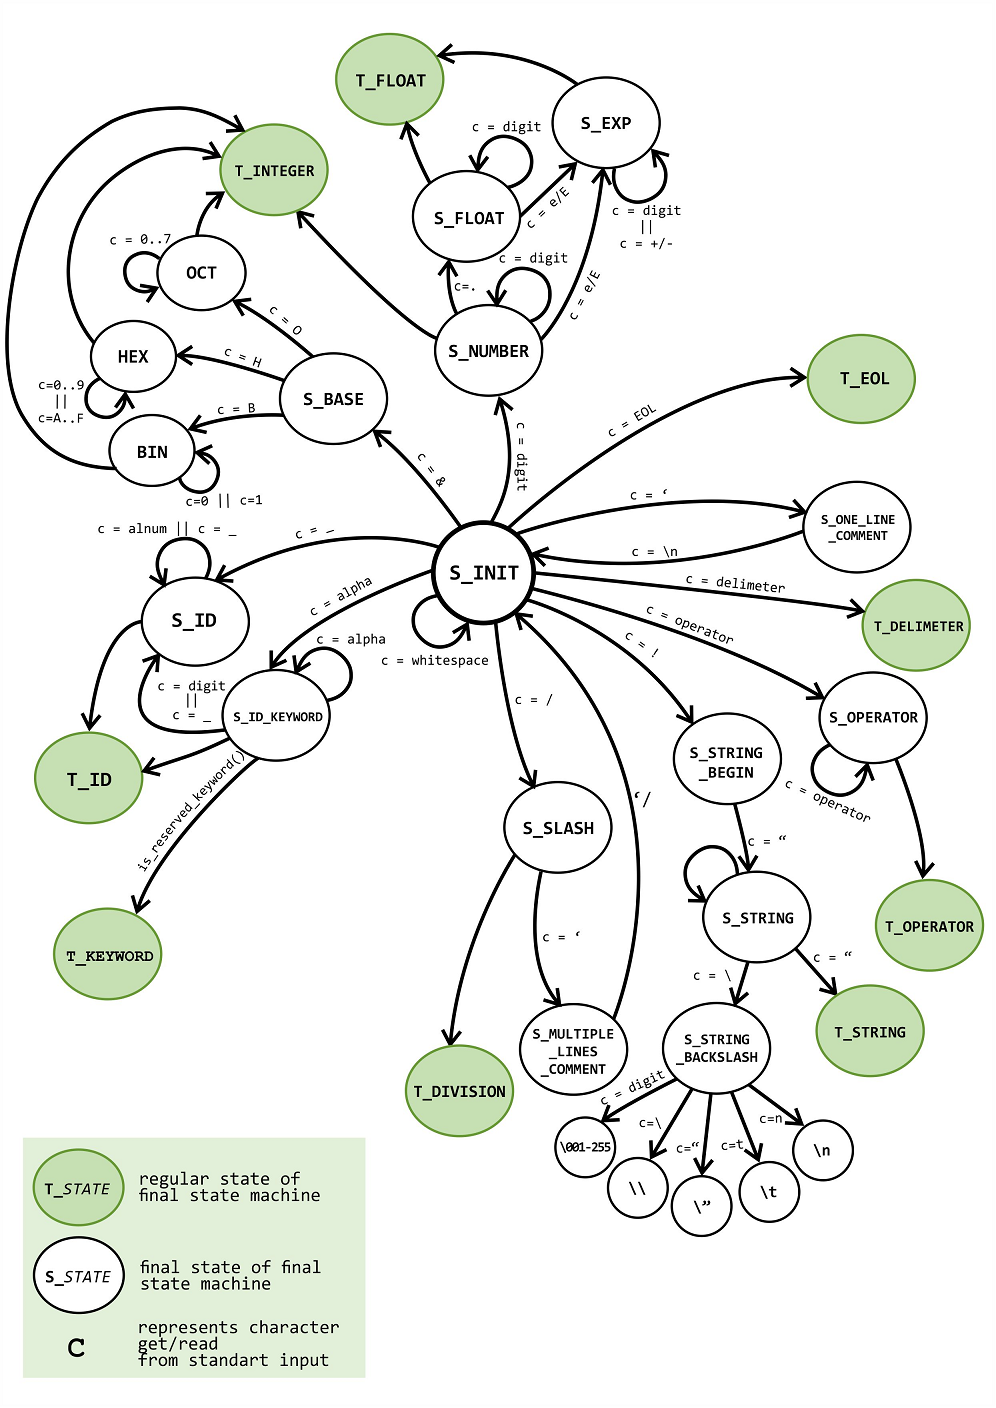
\includegraphics[height = 21cm]{FinalStateMachine.png}
		\end{figure}
		\subsection{LL-gramatika}

		1:  <S> -> <declaration-list> scope <statement-list> end scope \newline
		2:  <S> -> EOF \newline
		3:  <declaration-list> -> eps \newline
		4:  <declaration-list> -> T\_EOL  \newline
		5:  <declaration-list> -> dim T\_ID as <data-type> <assign> T\_EOL <declaration-list> \newline
		6:  <declaration-list> -> declare <function-decl> T\_EOL <declaration-list> \newline
		7:  <declaration-list> -> <function-decl> T\_EOL <statement-list> End Function T\_EOL <declaration-list> \newline
		8:  <function-decl> -> Function T\_ID ( <param-list> ) as <data-type> \newline
		9:  <data-type> -> Integer \newline
		10: <data-type> -> Double \newline
		11: <data-type> -> String \newline
		12: <assign> -> eps \newline
		13: <assign> -> = <E> \newline
		14: <param-list> -> <param> <next-param> \newline
		15: <param> -> T\_ID as <data-type> \newline
		16: <next-param> ->  \newline
		17: <next-param> -> , <param> <next-param> \newline
		18: <statement-list> -> <statement> T\_EOL <statement-list> \newline
		19: <statement-list> -> eps \newline
		20: <statement> -> eps \newline
		21: <statement> -> T\_ID <call-assign> \newline
		22: <statement> -> print <print-list> \newline
		23: <statement> -> input T\_ID \newline
		24: <statement> -> if <E> then T\_EOL <statement-list> else T\_EOL <statement-list> end if \newline
		25: <statement> -> do while <E> T\_EOL <statement-list> loop \newline
		26: <statement> -> return <E> \newline
		27: <call-assign> -> = <value> \newline
		28: <value> -> <E> \newline
		29: <value> -> T\_ID <call> \newline
		30: <call> -> ( <argument-list> ) \newline
		31: <argument-list> -> <E> <next-arg> \newline
		32: <next-arg> -> eps \newline
		33: <next-arg> -> , <E> <next-arg> \newline
		34: <print-list> -> <E> <next-print> \newline
		35: <next-print> -> eps \newline
		36: <next-print> -> ; <E> <next-print>  \newline
		37: <E> -> <E> op <E> \newline
		38: <E> -> ( <E> ) \newline

		\subsection{LL-tabulka}
		\begin{center}
			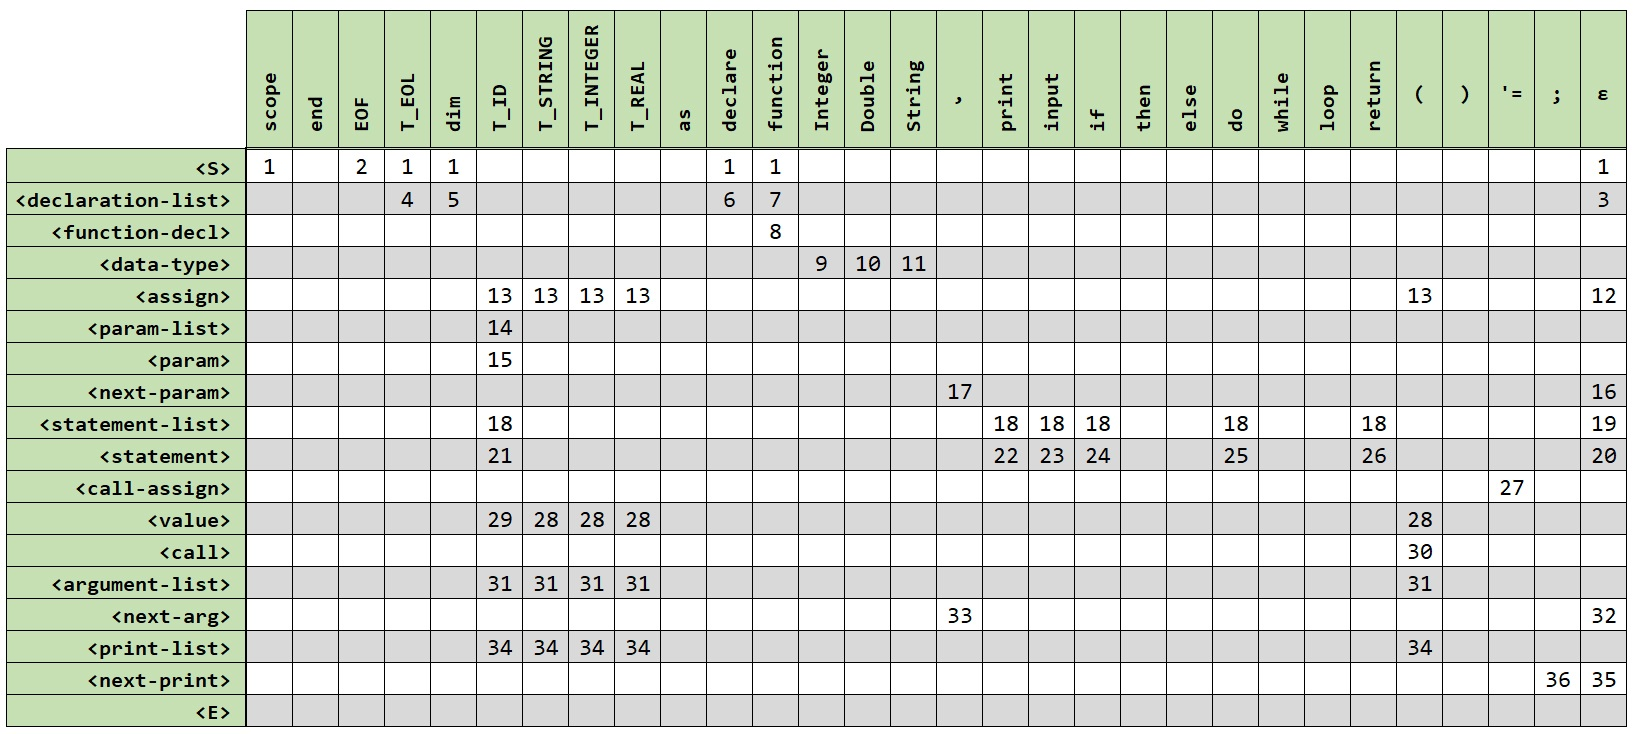
\includegraphics[height = 8 cm]{LL_tab.png}
		\end{center}
		\subsection{Precedenční tabulka}
		\begin{center}
			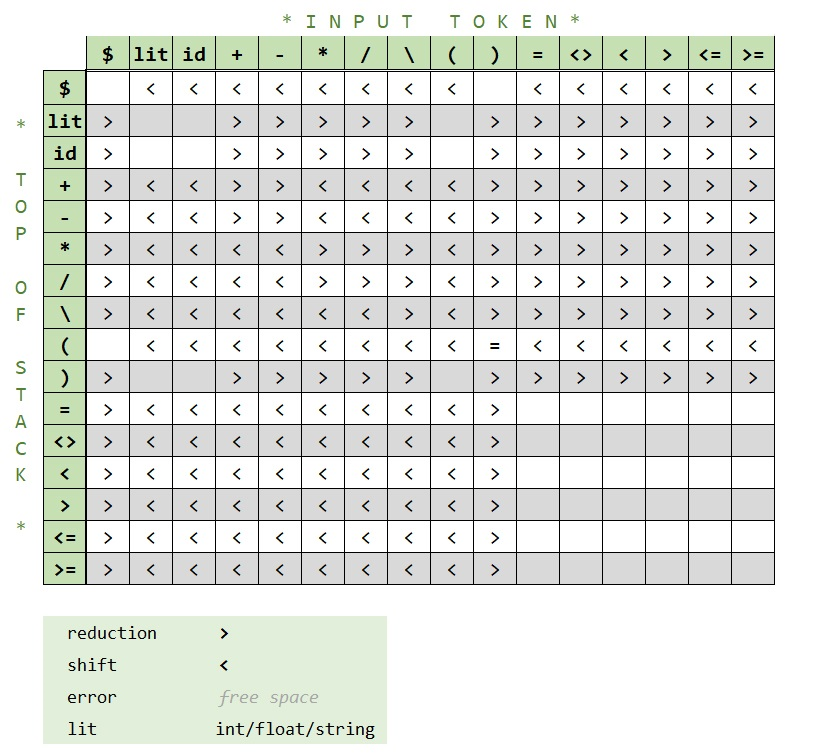
\includegraphics[height = 12 cm]{precedence_tab.png}
		\end{center}


\end{document}
